\documentclass[PhD-Yoann-Dupont.tex]{subfiles}
\begin{document}

Dans cette section, nous proposons une vue simplifiée du processus d'annotation. Nous nous sommes principalement basés sur la thèse de \citet{fort2012ressources} pour l'écriture de cette section.

Comme l'a souligné \citet{fort2012ressources}, une campagne d'annotation ne commence pas avec l'annotation elle-même, mais par l'identification des acteurs principaux dont chacun a un rôle précis à jouer. Elle distingue les rôles principaux suivants :

\begin{enumerate}
    \item \textbf{le ou les financier(s)}, qui fournit les fonds pour la campagne d'annotation et éventuellement son évaluation ;
    \item \textbf{le(s) client(s) ou donneur(s) d'ordre}, pour lesquels le corpus annoté répond à un besoin de plus haut niveau, comme créer ou évaluer des outils ;
    \item \textbf{le gestionnaire de la campagne}, qui doit s'assurer de la bonne mise-en-place et du bon déroulement de la campagne ;
    \item \textbf{le ou les annotateur(s) expert(s)}, des spécialistes du domaine, voire de la tâche, qui gère les annotateurs et feront au besoin l'adjudication du corpus ;
    \item \textbf{les annotateur(s)}, qui réalisent concrètement l'annotation ;
    \item \textbf{le ou les évaluateur(s)}, chargés d'évaluer la qualité du corpus annoté et/ou des outils d'intérêt pour les clients.
\end{enumerate}

Une fois ces rôles attribués (certaines personnes peuvent occuper plusieurs rôles, mais ce n'est pas sans risque), la première étape pour l'annotation d'un corpus consiste à établir un \emph{schéma d'annotation}. Ce schéma permet de déterminer trois éléments :

\begin{enumerate}
    \item ce qui est accessible à l'utilisateur, appelé le schéma externe. Il s'agit généralement de l'interface proposée par un logiciel d'annotation. Un exemple de logiciel pour l'annotation est GATE \citep{cunningham2002gate} et est illustré dans la figure \ref{fig:gate-annotation}.
    \item comment structurer les annotations. \citet{fort2012ressources} parle de la \emph{structure logique} du schéma d'annotation (appelée par ailleurs \emph{modèle}, \emph{schéma} ou \emph{format}). Il s'agit de la spécification de l'annotation d'un point de vue formel.
    \item comment stocker physiquement les annotations. Il s'agit en général du format de fichiers et la syntaxe de l'annotation. Deux exemples sont donnés dans la figure \ref{fig:inline-vs-standoff}.
\end{enumerate}

\begin{figure}[ht!]
    \centering
    \includegraphics[scale=0.66]{images/fort/GATE}
    \caption{Un exemple d'annotation avec l'outil GATE.}
    \label{fig:gate-annotation}
\end{figure}

Il existe deux grands méthodes d'annotation : les annotations insérées et les annotations déportées. Dans la méthode insérée, les annotations sont directement insérées dans le texte, a l'avantage d'être plus simple et d'offrir au lecteur l'annotation directement dans le texte, ce qui permet de visualiser humainement les annotations positionnées. La méthode déportée, où les annotations sont stockées en dehors du texte, permet une structuration plus simple des annotations et ne modifie pas le contenu textuel d'origine, mais peut s'avérer plus compliquée à replacer dans le texte. Des exemples sont donnés dans la figure \ref{fig:inline-vs-standoff}. Il n'existe pas vraiment de format standard universel, dans le sens où chaque logiciel utilise généralement son propre format en interne. Il existe cependant des formats standardisés, généralement utilisés dans un but d'échange (ils sont généralement convertis en format interne par un logiciel), parmi lesquels nous pouvons citer les recommandations TEI\footnote{il s'agit plus d'un guide où de nombreux éléments XML sont définis pour aider à la construction d'un type de document XML. Les recommandations TEI peuvent être utilisées différemments de projet en projet.} \citep{sperberg1994guidelines} ou le format BioC \citep{comeau2013bioc} pour les textes biomédicaux.

% \begin{figure}[ht!]
    % \centering
    % \lstset{language=XML}
    % \begin{lstlisting}[basicstyle=\scriptsize]
% <document>
  % <text>
    % <mention type="Person">Yoann Dupont</mention> fait une these a <mention type="Organisation">Paris 3</mention>.
  % </text>
% </document>\end{lstlisting}
    % \begin{lstlisting}[basicstyle=\scriptsize]
% <document>
  % <text>Yoann Dupont fait une these a Paris 3.</text>
  % <mention type="Person" start="0" length="12" />
  % <mention type="Organisation" start="0" length="7" />
% </document>\end{lstlisting}
% \caption{Un exemple d'annotation insérée et un équivalent déporté au format XML.}
% \label{fig:inline-vs-standoff}
% \end{figure}

\begin{figure}[ht!]
\footnotesize
\begin{xml}\xmarker{document}{}{\xmarker{text}{}{\\
    \xmarker{mention}{ \xfield{type}{Person}}{Yoann Dupont} fait une thèse à\\
\xmarker{mention}{ \xfield{type}{Organisation}}{Paris 3}.}\\
}\end{xml}
~
\begin{xml}\xmarker{document}{}{\\
  \xmarker{text}{}{Yoann Dupont fait une thèse a Paris 3.}\\
  \xunit{mention}{\xfield{type}{Person} \xfield{start}{0} \xfield{length}{12}}\\
  \xunit{mention}{\xfield{type}{Organisation} \xfield{start}{30} \xfield{length}{7}}\\
}\end{xml}
\caption{Un exemple d'annotation insérée et un équivalent déporté au format XML.}
\label{fig:inline-vs-standoff}
\end{figure}

Ce schéma doit être établi avant le début du travail des annotateurs et doit être figé une fois le processus d'annotation commencé, au risque de donner un résultat incohérent. Un guide d'annotation doit être fourni, il s'agit d'un fichier expliquant ce que représente chaque entité et ce qui doit ou non être annoté comme tel. Ce fichier devra être utilisé par les annotateurs afin de comprendre la tâche telle qu'elle est prévue et de les aider en cas d'interrogation.

La création d'un guide d'annotation se fait à l'aide d'une mini-campagne de préannotation par un expert. Elle permet de voir les premiers problèmes liés à la tâche et de fournir les directions générales à utiliser de manière concrète. Ce guide d'annotation sera ensuite mis à jour au début de la campagne d'annotation afin de prendre en compte les retours des annotateurs.

Une fois l'annotation du corpus finie, la campagne d'annotation passe alors dans la passe de finalisation. Si le corpus est jugé dans un état suffisamment bon, il peut d'emblée être publié. Si des corrections sont jugées nécessaires, les annotations fournies par les différents annotateurs sont passées en revue et corrigées avant la diffusion. Cette phase s'appelle l'\emph{adjudication} du corpus. Il n'est pas impossible cependant que la campagne se soit mal passée et que le corpus ne soit pas exploitable dans un but applicatif, auquel cas il ne sera pas diffusé, menant à l'échec de la campagne d'annotation.

\begin{figure}[ht!]
    \centering
    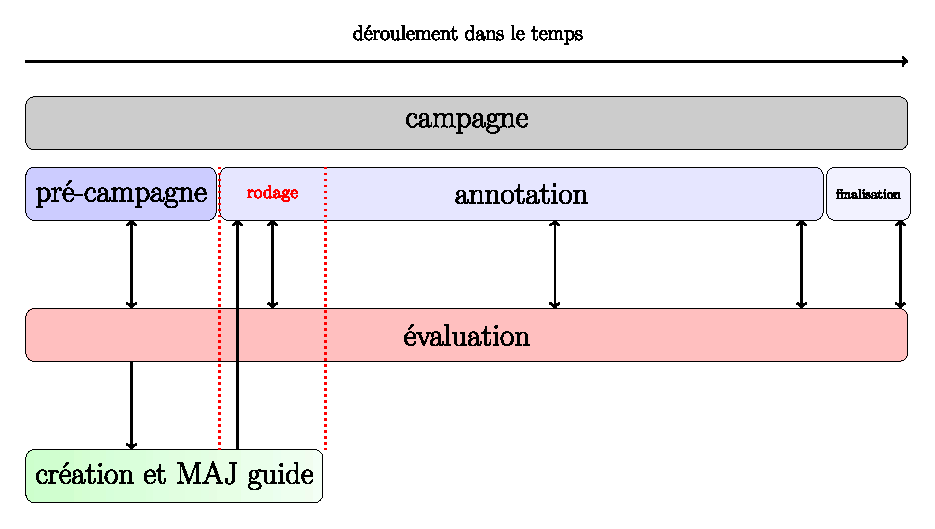
\includegraphics[scale=1.0]{images/fort/campaign}
    \caption{Organisation générale d'une campagne d'annotation. Image reprise de \citet{fort2012ressources}}
    \label{fig:campaign-organisation}
\end{figure}

Une étape importante de la campagne d'annotation consiste à évaluer le travail réalisé par les annotateurs. Notamment, la mesure de leur accord permet de donner une idée de la consistance des annotations, donc de la reproductibilité de leur travail par des outils de TAL.

\end{document}